\documentclass[]{article}
\usepackage{lmodern}
\usepackage{amssymb,amsmath}
\usepackage{ifxetex,ifluatex}
\usepackage{fixltx2e} % provides \textsubscript
\ifnum 0\ifxetex 1\fi\ifluatex 1\fi=0 % if pdftex
  \usepackage[T1]{fontenc}
  \usepackage[utf8]{inputenc}
\else % if luatex or xelatex
  \ifxetex
    \usepackage{mathspec}
    \usepackage{xltxtra,xunicode}
  \else
    \usepackage{fontspec}
  \fi
  \defaultfontfeatures{Mapping=tex-text,Scale=MatchLowercase}
  \newcommand{\euro}{€}
\fi
% use upquote if available, for straight quotes in verbatim environments
\IfFileExists{upquote.sty}{\usepackage{upquote}}{}
% use microtype if available
\IfFileExists{microtype.sty}{%
\usepackage{microtype}
\UseMicrotypeSet[protrusion]{basicmath} % disable protrusion for tt fonts
}{}
\usepackage[margin=1in]{geometry}
\usepackage{color}
\usepackage{fancyvrb}
\newcommand{\VerbBar}{|}
\newcommand{\VERB}{\Verb[commandchars=\\\{\}]}
\DefineVerbatimEnvironment{Highlighting}{Verbatim}{commandchars=\\\{\}}
% Add ',fontsize=\small' for more characters per line
\usepackage{framed}
\definecolor{shadecolor}{RGB}{248,248,248}
\newenvironment{Shaded}{\begin{snugshade}}{\end{snugshade}}
\newcommand{\KeywordTok}[1]{\textcolor[rgb]{0.13,0.29,0.53}{\textbf{{#1}}}}
\newcommand{\DataTypeTok}[1]{\textcolor[rgb]{0.13,0.29,0.53}{{#1}}}
\newcommand{\DecValTok}[1]{\textcolor[rgb]{0.00,0.00,0.81}{{#1}}}
\newcommand{\BaseNTok}[1]{\textcolor[rgb]{0.00,0.00,0.81}{{#1}}}
\newcommand{\FloatTok}[1]{\textcolor[rgb]{0.00,0.00,0.81}{{#1}}}
\newcommand{\CharTok}[1]{\textcolor[rgb]{0.31,0.60,0.02}{{#1}}}
\newcommand{\StringTok}[1]{\textcolor[rgb]{0.31,0.60,0.02}{{#1}}}
\newcommand{\CommentTok}[1]{\textcolor[rgb]{0.56,0.35,0.01}{\textit{{#1}}}}
\newcommand{\OtherTok}[1]{\textcolor[rgb]{0.56,0.35,0.01}{{#1}}}
\newcommand{\AlertTok}[1]{\textcolor[rgb]{0.94,0.16,0.16}{{#1}}}
\newcommand{\FunctionTok}[1]{\textcolor[rgb]{0.00,0.00,0.00}{{#1}}}
\newcommand{\RegionMarkerTok}[1]{{#1}}
\newcommand{\ErrorTok}[1]{\textbf{{#1}}}
\newcommand{\NormalTok}[1]{{#1}}
\usepackage{graphicx}
\makeatletter
\def\maxwidth{\ifdim\Gin@nat@width>\linewidth\linewidth\else\Gin@nat@width\fi}
\def\maxheight{\ifdim\Gin@nat@height>\textheight\textheight\else\Gin@nat@height\fi}
\makeatother
% Scale images if necessary, so that they will not overflow the page
% margins by default, and it is still possible to overwrite the defaults
% using explicit options in \includegraphics[width, height, ...]{}
\setkeys{Gin}{width=\maxwidth,height=\maxheight,keepaspectratio}
\ifxetex
  \usepackage[setpagesize=false, % page size defined by xetex
              unicode=false, % unicode breaks when used with xetex
              xetex]{hyperref}
\else
  \usepackage[unicode=true]{hyperref}
\fi
\hypersetup{breaklinks=true,
            bookmarks=true,
            pdfauthor={},
            pdftitle={Reproducible Research Peer Assessment 1},
            colorlinks=true,
            citecolor=blue,
            urlcolor=blue,
            linkcolor=magenta,
            pdfborder={0 0 0}}
\urlstyle{same}  % don't use monospace font for urls
\setlength{\parindent}{0pt}
\setlength{\parskip}{6pt plus 2pt minus 1pt}
\setlength{\emergencystretch}{3em}  % prevent overfull lines
\setcounter{secnumdepth}{0}

%%% Change title format to be more compact
\usepackage{titling}
\setlength{\droptitle}{-2em}
  \title{Reproducible Research Peer Assessment 1}
  \pretitle{\vspace{\droptitle}\centering\huge}
  \posttitle{\par}
  \author{}
  \preauthor{}\postauthor{}
  \date{}
  \predate{}\postdate{}




\begin{document}

\maketitle


\subsection{Loading and preprocessing the
data}\label{loading-and-preprocessing-the-data}

\begin{Shaded}
\begin{Highlighting}[]
\NormalTok{data <-}\StringTok{ }\KeywordTok{read.csv}\NormalTok{(}\KeywordTok{unz}\NormalTok{(}\StringTok{"activity.zip"}\NormalTok{,}\StringTok{"activity.csv"}\NormalTok{))}

\NormalTok{data_unaltered <-}\StringTok{ }\KeywordTok{read.csv}\NormalTok{(}\KeywordTok{unz}\NormalTok{(}\StringTok{"activity.zip"}\NormalTok{,}\StringTok{"activity.csv"}\NormalTok{))}

\NormalTok{data_type<-}\KeywordTok{as.Date}\NormalTok{(data$date,}\StringTok{"%Y-%m-%d"}\NormalTok{)}

\NormalTok{data$time_type <-}\StringTok{ }\NormalTok{data_type}


\NormalTok{newdata<-}\StringTok{ }\NormalTok{data[}\KeywordTok{complete.cases}\NormalTok{(data),]}
\end{Highlighting}
\end{Shaded}

\subsection{What is mean total number of steps taken per
day?}\label{what-is-mean-total-number-of-steps-taken-per-day}

\begin{Shaded}
\begin{Highlighting}[]
\NormalTok{totalstepsperday <-}\StringTok{ }\KeywordTok{aggregate}\NormalTok{(newdata$steps,}\DataTypeTok{by=}\KeywordTok{list}\NormalTok{(newdata$time_type),}\DataTypeTok{FUN=}\NormalTok{sum)}
\NormalTok{meantotalperday <-}\KeywordTok{aggregate}\NormalTok{(newdata$steps,}\DataTypeTok{by=}\KeywordTok{list}\NormalTok{(newdata$time_type),}\DataTypeTok{FUN=}\NormalTok{mean)}


\NormalTok{meanperday <-}\KeywordTok{mean}\NormalTok{(totalstepsperday$x)}
\NormalTok{meanperday}
\end{Highlighting}
\end{Shaded}

\begin{verbatim}
## [1] 10766.19
\end{verbatim}

\begin{Shaded}
\begin{Highlighting}[]
\NormalTok{medianperday <-}\StringTok{ }\KeywordTok{median}\NormalTok{(totalstepsperday$x)}
\NormalTok{medianperday}
\end{Highlighting}
\end{Shaded}

\begin{verbatim}
## [1] 10765
\end{verbatim}

\begin{Shaded}
\begin{Highlighting}[]
\NormalTok{val<-}\StringTok{ }\KeywordTok{as.character}\NormalTok{(meanperday)}
\NormalTok{val2 <-}\StringTok{ }\NormalTok{medianperday}
\end{Highlighting}
\end{Shaded}

the mean is 10766.1886792453 the median is 10765

The histogram

\begin{Shaded}
\begin{Highlighting}[]
\KeywordTok{hist}\NormalTok{(totalstepsperday$x,}\DataTypeTok{xlab=}\StringTok{"Steps per day"}\NormalTok{)}
\end{Highlighting}
\end{Shaded}

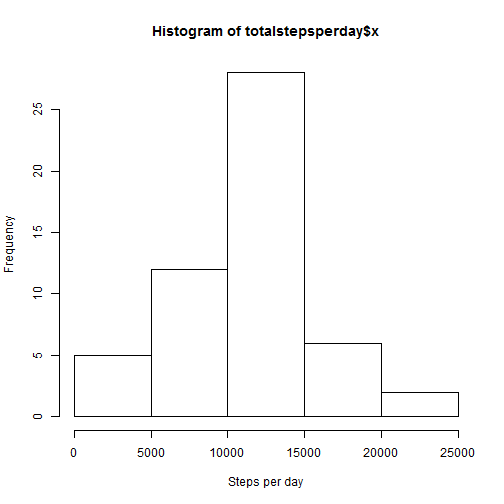
\includegraphics{PA1_template_files/figure-latex/unnamed-chunk-3-1.pdf}

\begin{Shaded}
\begin{Highlighting}[]
\NormalTok{mediantotalperday <-}\KeywordTok{aggregate}\NormalTok{(newdata$steps,}\DataTypeTok{by=}\KeywordTok{list}\NormalTok{(newdata$time_type),}\DataTypeTok{FUN=}\NormalTok{median)}

\NormalTok{newdata2 <-meantotalperday}
\NormalTok{newdata2$median <-}\StringTok{ }\NormalTok{mediantotalperday$x}
\KeywordTok{colnames}\NormalTok{(newdata2)[}\DecValTok{2}\NormalTok{]<-}\StringTok{"Meantotalperday"}
\KeywordTok{colnames}\NormalTok{(newdata2)[}\DecValTok{1}\NormalTok{]<-}\StringTok{"Date"}
\KeywordTok{print}\NormalTok{(newdata2)}
\end{Highlighting}
\end{Shaded}

\begin{verbatim}
##          Date Meantotalperday median
## 1  2012-10-02       0.4375000      0
## 2  2012-10-03      39.4166667      0
## 3  2012-10-04      42.0694444      0
## 4  2012-10-05      46.1597222      0
## 5  2012-10-06      53.5416667      0
## 6  2012-10-07      38.2465278      0
## 7  2012-10-09      44.4826389      0
## 8  2012-10-10      34.3750000      0
## 9  2012-10-11      35.7777778      0
## 10 2012-10-12      60.3541667      0
## 11 2012-10-13      43.1458333      0
## 12 2012-10-14      52.4236111      0
## 13 2012-10-15      35.2048611      0
## 14 2012-10-16      52.3750000      0
## 15 2012-10-17      46.7083333      0
## 16 2012-10-18      34.9166667      0
## 17 2012-10-19      41.0729167      0
## 18 2012-10-20      36.0937500      0
## 19 2012-10-21      30.6284722      0
## 20 2012-10-22      46.7361111      0
## 21 2012-10-23      30.9652778      0
## 22 2012-10-24      29.0104167      0
## 23 2012-10-25       8.6527778      0
## 24 2012-10-26      23.5347222      0
## 25 2012-10-27      35.1354167      0
## 26 2012-10-28      39.7847222      0
## 27 2012-10-29      17.4236111      0
## 28 2012-10-30      34.0937500      0
## 29 2012-10-31      53.5208333      0
## 30 2012-11-02      36.8055556      0
## 31 2012-11-03      36.7048611      0
## 32 2012-11-05      36.2465278      0
## 33 2012-11-06      28.9375000      0
## 34 2012-11-07      44.7326389      0
## 35 2012-11-08      11.1770833      0
## 36 2012-11-11      43.7777778      0
## 37 2012-11-12      37.3784722      0
## 38 2012-11-13      25.4722222      0
## 39 2012-11-15       0.1423611      0
## 40 2012-11-16      18.8923611      0
## 41 2012-11-17      49.7881944      0
## 42 2012-11-18      52.4652778      0
## 43 2012-11-19      30.6979167      0
## 44 2012-11-20      15.5277778      0
## 45 2012-11-21      44.3993056      0
## 46 2012-11-22      70.9270833      0
## 47 2012-11-23      73.5902778      0
## 48 2012-11-24      50.2708333      0
## 49 2012-11-25      41.0902778      0
## 50 2012-11-26      38.7569444      0
## 51 2012-11-27      47.3819444      0
## 52 2012-11-28      35.3576389      0
## 53 2012-11-29      24.4687500      0
\end{verbatim}

\subsection{What is the average daily activity
pattern?}\label{what-is-the-average-daily-activity-pattern}

\begin{Shaded}
\begin{Highlighting}[]
\NormalTok{averagenumberofstpes<-}\KeywordTok{aggregate}\NormalTok{(newdata$steps,}\DataTypeTok{by=}\KeywordTok{list}\NormalTok{(newdata$interval),}\DataTypeTok{FUN=}\NormalTok{mean)}
\KeywordTok{plot}\NormalTok{(averagenumberofstpes$Group}\FloatTok{.1}\NormalTok{,averagenumberofstpes$x,}\DataTypeTok{xlab=}\StringTok{"interval"}\NormalTok{,}\DataTypeTok{ylab=}\StringTok{"AverageNumberofSteps"}\NormalTok{,}\DataTypeTok{type=}\StringTok{"l"}\NormalTok{)}
\end{Highlighting}
\end{Shaded}

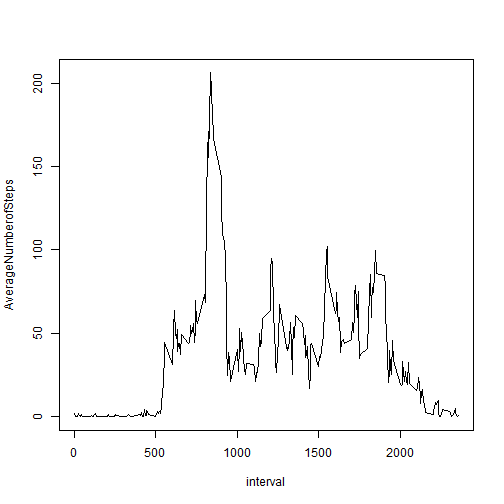
\includegraphics{PA1_template_files/figure-latex/unnamed-chunk-4-1.pdf}

\begin{Shaded}
\begin{Highlighting}[]
\NormalTok{interval<-averagenumberofstpes[averagenumberofstpes$x==}\KeywordTok{max}\NormalTok{(averagenumberofstpes$x),]$Group}\FloatTok{.1}
\KeywordTok{print}\NormalTok{(interval)}
\end{Highlighting}
\end{Shaded}

\begin{verbatim}
## [1] 835
\end{verbatim}

\subsection{Imputing missing values}\label{imputing-missing-values}

\begin{Shaded}
\begin{Highlighting}[]
\NormalTok{newdata3<-}\StringTok{ }\NormalTok{data[!}\KeywordTok{complete.cases}\NormalTok{(data),]}
\NormalTok{missingrows<-}\KeywordTok{nrow}\NormalTok{(newdata3)}
\KeywordTok{print}\NormalTok{(missingrows)}
\end{Highlighting}
\end{Shaded}

\begin{verbatim}
## [1] 2304
\end{verbatim}

\begin{Shaded}
\begin{Highlighting}[]
\NormalTok{data[!}\KeywordTok{complete.cases}\NormalTok{(data),]$steps=}\DecValTok{1}
\NormalTok{totalstepsperday2 <-}\StringTok{ }\KeywordTok{aggregate}\NormalTok{(data$steps,}\DataTypeTok{by=}\KeywordTok{list}\NormalTok{(data$time_type),}\DataTypeTok{FUN=}\NormalTok{sum)}
\NormalTok{meantotalperday2 <-}\KeywordTok{aggregate}\NormalTok{(data$steps,}\DataTypeTok{by=}\KeywordTok{list}\NormalTok{(data$time_type),}\DataTypeTok{FUN=}\NormalTok{mean)}
\KeywordTok{hist}\NormalTok{(totalstepsperday2$x,}\DataTypeTok{xlab=}\StringTok{"Steps per day"}\NormalTok{)}
\end{Highlighting}
\end{Shaded}

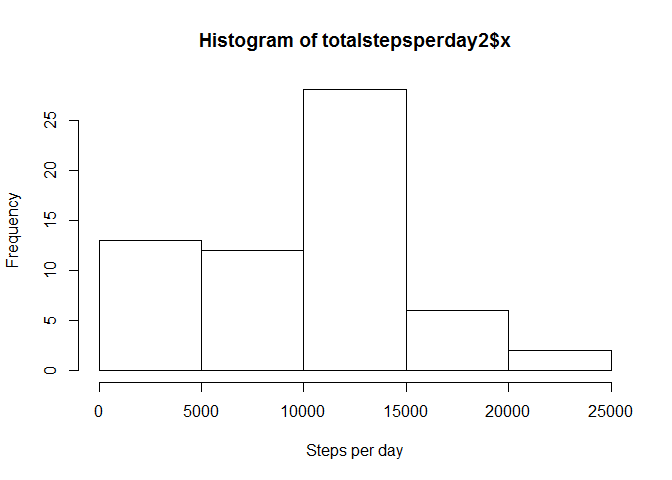
\includegraphics{PA1_template_files/figure-latex/unnamed-chunk-5-1.pdf}

\begin{Shaded}
\begin{Highlighting}[]
\NormalTok{mediantotalperday2 <-}\KeywordTok{aggregate}\NormalTok{(data$steps,}\DataTypeTok{by=}\KeywordTok{list}\NormalTok{(data$time_type),}\DataTypeTok{FUN=}\NormalTok{median)}



\NormalTok{newdata5 <-meantotalperday2}
\NormalTok{newdata5$median <-}\StringTok{ }\NormalTok{mediantotalperday2$x}
\KeywordTok{colnames}\NormalTok{(newdata5)[}\DecValTok{2}\NormalTok{]<-}\StringTok{"Meantotalperday"}
\KeywordTok{colnames}\NormalTok{(newdata5)[}\DecValTok{1}\NormalTok{]<-}\StringTok{"Date"}
\KeywordTok{print}\NormalTok{(newdata5)}
\end{Highlighting}
\end{Shaded}

\begin{verbatim}
##          Date Meantotalperday median
## 1  2012-10-01       1.0000000      1
## 2  2012-10-02       0.4375000      0
## 3  2012-10-03      39.4166667      0
## 4  2012-10-04      42.0694444      0
## 5  2012-10-05      46.1597222      0
## 6  2012-10-06      53.5416667      0
## 7  2012-10-07      38.2465278      0
## 8  2012-10-08       1.0000000      1
## 9  2012-10-09      44.4826389      0
## 10 2012-10-10      34.3750000      0
## 11 2012-10-11      35.7777778      0
## 12 2012-10-12      60.3541667      0
## 13 2012-10-13      43.1458333      0
## 14 2012-10-14      52.4236111      0
## 15 2012-10-15      35.2048611      0
## 16 2012-10-16      52.3750000      0
## 17 2012-10-17      46.7083333      0
## 18 2012-10-18      34.9166667      0
## 19 2012-10-19      41.0729167      0
## 20 2012-10-20      36.0937500      0
## 21 2012-10-21      30.6284722      0
## 22 2012-10-22      46.7361111      0
## 23 2012-10-23      30.9652778      0
## 24 2012-10-24      29.0104167      0
## 25 2012-10-25       8.6527778      0
## 26 2012-10-26      23.5347222      0
## 27 2012-10-27      35.1354167      0
## 28 2012-10-28      39.7847222      0
## 29 2012-10-29      17.4236111      0
## 30 2012-10-30      34.0937500      0
## 31 2012-10-31      53.5208333      0
## 32 2012-11-01       1.0000000      1
## 33 2012-11-02      36.8055556      0
## 34 2012-11-03      36.7048611      0
## 35 2012-11-04       1.0000000      1
## 36 2012-11-05      36.2465278      0
## 37 2012-11-06      28.9375000      0
## 38 2012-11-07      44.7326389      0
## 39 2012-11-08      11.1770833      0
## 40 2012-11-09       1.0000000      1
## 41 2012-11-10       1.0000000      1
## 42 2012-11-11      43.7777778      0
## 43 2012-11-12      37.3784722      0
## 44 2012-11-13      25.4722222      0
## 45 2012-11-14       1.0000000      1
## 46 2012-11-15       0.1423611      0
## 47 2012-11-16      18.8923611      0
## 48 2012-11-17      49.7881944      0
## 49 2012-11-18      52.4652778      0
## 50 2012-11-19      30.6979167      0
## 51 2012-11-20      15.5277778      0
## 52 2012-11-21      44.3993056      0
## 53 2012-11-22      70.9270833      0
## 54 2012-11-23      73.5902778      0
## 55 2012-11-24      50.2708333      0
## 56 2012-11-25      41.0902778      0
## 57 2012-11-26      38.7569444      0
## 58 2012-11-27      47.3819444      0
## 59 2012-11-28      35.3576389      0
## 60 2012-11-29      24.4687500      0
## 61 2012-11-30       1.0000000      1
\end{verbatim}

As can be seen in the histogram graph, the profiles change significantly
between the first and second histogram. for the mean values, the
difference is not so large FOr the median value, it shows in the table
that it takes the value of the replacement

\subsection{Are there differences in activity patterns between weekdays
and
weekends?}\label{are-there-differences-in-activity-patterns-between-weekdays-and-weekends}

\begin{Shaded}
\begin{Highlighting}[]
\NormalTok{dataWorWekend <-}\KeywordTok{c}\NormalTok{(}\StringTok{"Wekend"}\NormalTok{,}\StringTok{"Week"}\NormalTok{,}\StringTok{"Week"}\NormalTok{,}\StringTok{"Week"}\NormalTok{,}\StringTok{"Week"}\NormalTok{,}\StringTok{"Week"}\NormalTok{,}\StringTok{"Wekend"}\NormalTok{)[}\KeywordTok{as.POSIXlt}\NormalTok{(data$time_type)$wday}\DecValTok{+1}\NormalTok{]}


\NormalTok{data$dataWorWekend <-}\StringTok{ }\NormalTok{dataWorWekend }
\NormalTok{meantotalstepperday3 <-}\KeywordTok{aggregate}\NormalTok{(data$steps,}\DataTypeTok{by=}\KeywordTok{list}\NormalTok{(data$time_type,data$dataWorWekend,data$interval),}\DataTypeTok{FUN=}\NormalTok{mean)}

\NormalTok{f <-}\StringTok{ }\KeywordTok{factor}\NormalTok{(meantotalstepperday3$Group}\FloatTok{.2}\NormalTok{,}\DataTypeTok{labels=}\KeywordTok{c}\NormalTok{(}\StringTok{"weekend"}\NormalTok{,}\StringTok{"weekday"}\NormalTok{))}

\KeywordTok{library}\NormalTok{(lattice)}

\KeywordTok{xyplot}\NormalTok{(meantotalstepperday3$x ~}\StringTok{ }\NormalTok{meantotalstepperday3$Group}\FloatTok{.3} \NormalTok{|}\StringTok{ }\NormalTok{f, }\DataTypeTok{layout=}\KeywordTok{c}\NormalTok{(}\DecValTok{1}\NormalTok{,}\DecValTok{2}\NormalTok{),}\DataTypeTok{type=}\StringTok{'l'}\NormalTok{)}
\end{Highlighting}
\end{Shaded}

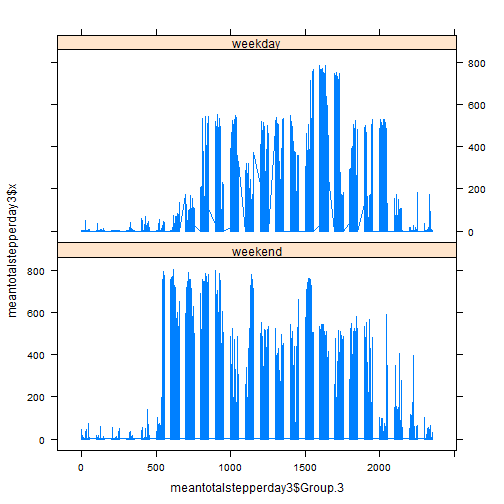
\includegraphics{PA1_template_files/figure-latex/unnamed-chunk-6-1.pdf}

As seen from the graph, there is a slight difference between the average
number of steps between the weekday and the weekend.

\end{document}
